\section{La economía descentralizada}

\subsection{Motivación del modelo de equilibrio general}

Los modelos de equilibrio parcial buscan describir los ajustes de oferta y demanda de un mercado específico tratando el resto de la economía como constante. Estos modelos de equilibrio parcial fueron desarrollados en gran parte por \textbf{Alfred Marshall}.\marginnote{\textbf{Alfred Marshall:} Economista británico que durante finales del siglo XIX traslapó conceptos de la economía clásica con la escuela marginalista.}[-2cm] Por ejemplo, si analizaramos el mercado de manzanas supondríamos que los costos de los factores de producción son exógenos, esto significaría que los costes de trabajo (salarios) se mantendrían constantes independiente de la dotación y equilibrio del modelo. 

Encontrándose el precio de mercado en equilibrio, en ninguna extensión se aborda el equilibrio del mercado laboral que hay detrás de la producción de manzanas. En la realidad como distintos mercados están interactuando constantemente un shock en un mercado puede derivar a múltiples ajustes en mercados relacionados. Por ejemplo, un subsidio al empleo bajaría los costes por trabajo, potencialmente aumentando la producción de manzanas. Estos fenómenos no se pueden analizar con modelos de equilibrio parcial pues se limitan a un sólo mercado dejando los factores como constantes dadas. 

Por otro lado, los modelos de \textbf{equilibrio general}\marginnote{\textbf{Equilibrio General:} Modelo que busca explicar el equilibrio dentro de una economía con más de un mercado en constante interacción.}[-1cm] describen dos o más mercados relacionados que se ajustan al mismo tiempo, lo cual nos podría dar una imagen más completa de los efectos de distintos shocks en la economía como un todo. Analizar el equilibrio de un número arbitrario de mercados es complejo, por suerte limitarnos a dos mercados y plantear diversos supuestos nos permite aun así, abstraer las conclusiones que encontramos relevantes para esta ocasión. 

\subsection{Planteamiento del modelo}

Una razón poderosa por la que limitarnos a analizar solo dos mercados es la \textbf{Ley de Walras}.\marginnote{\textbf{Ley de Walras:} En una economía de $n$ mercados, que $n-1$ de ellos esté en equilibrio implica que el otro también lo estará.}[-1cm] La ley de Walras es un principio desarrollado por \textbf{León Walras}\marginnote{\textbf{León Walras:} Economista francés de la escuela (neoclásica) de Lausana. Considerado fundador de la economía matemática.}[3cm] que plantea que al tener dos mercados, si el exceso de demanda de un bien es cero implica que el exceso de demanda del otro bien también será cero. Por lo tanto, los dos mercados están en equilibrio.\footnote{Con exceso de demanda igual a cero entiéndase como oferta igual a demanda.} Generalizando, si en una economía de $n$ mercados hay $n-1$ mercados en equilibrio, entonces el último mercado (el n-ésimo) también estará en equilibrio. Es por esto que limitarnos a analizar sólo dos mercados no influye mucho en las conclusiones relevantes del modelo. 

Vamos a describir una economía de intercambio entre dos individuos que al consumir dos bienes se formarán dos mercados. Estos individuos serán racionales, maximizarán su función de utilidad sujeto a una restricción presupuestaria.\footnote{Se asume que la función de utilidad es del tipo $u_i: \mathbb{R}_+^2 \xrightarrow{} \mathbb{R}$, la cual cumple con ser (i) continua, (ii) creciente y (iii) cóncava.} Cada agente tendrá una dotación inicial de bienes que podrá consumir e intercambiar. La restricción presupuestaria de cada individuo será determinada por su dotación inicial y el precio de mercado de los bienes que se le haya dotado. Mientras que los precios serán determinados entonces por la demanda (preferencias y poder adquisitivo) y la oferta (dotación total de los bienes). En particular vamos a asumir:

\begin{enumerate}
    \item No hay poder de mercado, los dos agentes en la economía serán tomadores de precios. 
    \item Información completa. Los dos individuos están al tanto de los bienes que hay en la economía, su cantidad y utilidad que les proporciona tanto a el como al otro. 
    \item No hay costos de transacción. 
    \item No hay externalidades. El consumo de un bien no afecta la utilidad de un externo de ninguna manera.\footnote{Este supuesto se puede levantar y llevar al mismo resultado de equilibrio bajo ciertas condiciones, asumiremos que no existe tal posibilidad.} 
\end{enumerate}

Los individuos comerciarán su dotación inicial arbitrariamente asignada llegando a una dotación que sea eficiente. Es intuitivo entender que un individuo solo intercambiará una cantidad de un bien mientras que el bien que le llegue a cambio le genere una utilidad mayor, solo accederan a intercambiar si son más felices con el acuerdo. Por lo tanto, habrá un punto en que dejarán de intercambiarse puesto que se agotaron todas las transacciones posibles, en este equilibrio ninguno de los dos puede estar mejor sin perjudicar al otro.

Este equilibrio se encuentra dentro de lo que se conoce como \textbf{equilibrio walrasiano}.\footnote{También se le llama equilibrio competitivo, fue introducido por Kenneth Arrow and Gérard Debreu a principios de los 50. (Requiere cita)}\marginnote{\textbf{Equilibrio Walrasiano:} Equilibrio de un mercado competitivo, la demanda y oferta de todos los bienes en la economía son iguales.}[-15cm] Cada individuo consumirá con respecto a su restricción, el resultado es que la demanda y la oferta se igualarán, de aquí se suele decir que se \textit{vacía el mercado}. En lo que sigue formalizaremos y pondremos nombre al proceso que se acaba de mencionar.

\subsection{Caja de Edgeworth}

La \textbf{Caja de Edgeworth}\marginnote{\textbf{Caja de Edgeworth:} Herramienta gráfica para representar un modelo de equilibrio general.}[-10cm] será la representación gráfica del modelo. Esta herramienta fue desarrollada por \textbf{Francis Edgeworth}\marginnote{\textbf{Francis Edgeworth:} Economista y estadístico británico que propone las curvas de indiferencia y caja de Edgeworth.}[-7cm] y \textbf{Arthur Bowley},\marginnote{\textbf{Arthur Bowley:} Economista y estadístico británico pionero de usar técnicas de muestreo en encuestas sociales.}[-2cm] economistas y estadísticos británicos. Las dimensiones de esta caja obedecerán a las dotaciones totales de cada bien. 

Esta economía considera dos individuos $i \in A,B$ que se intercambian dos bienes $j \in x,y$. Las dotaciones de bienes que tenga cada individuo se puede describir como un vector $\in \mathbb{R}^2_+$, más precisamente las dotaciones para un individuo $i$ serán:
\begin{equation*}
    \omega_i = (\omega_{ix} , \omega_{iy}) \in \mathbb{R}^2_+
\end{equation*}
En la figura \ref{fig:caja dimensiones} podemos observar que las dimensiones de la caja son $\omega_x = \omega_{Ax} + \omega_{Bx}$ por un lado y $\omega_y = \omega_{Ay} + \omega_{By}$ por el otro. Donde además ubicamos una la dotación inicial como un punto dentro de la caja $\omega^E \in \mathbb{R}^2_+$.
\begin{figure}
    \centering
    \caption{Dimensiones de la caja de Edgeworth}
    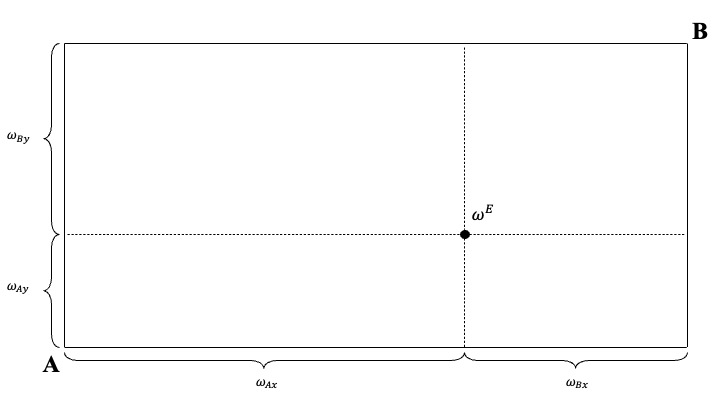
\includegraphics[width=\textwidth]{Figuras/EG Dotacion inicial.jpeg}
    \label{fig:caja dimensiones}
\end{figure}
Los mercados se encargarán de asignar precios a cada bien dadas las preferencias y dotaciones, estos precios los podemos denotar como un vector $p = (p_x, p_y) \in \mathbb{R}^2_+$. Para el individuo $i$ la riqueza se puede denotar como la cantidad de un bien ponderado por su precio: 
\begin{equation*}
    R_i = p_x \cdot \omega_{ix} + p_y \cdot \omega_{iy}
\end{equation*}
La riqueza vendrá siendo la restricción presupuestaria a la que está sujeta la maximización de utilidad. Es decir, el individuo $i$ maximizará su función $u: \mathbb{R}^2_+ \xrightarrow{} \mathbb{R}_+$ en este caso del tipo Cobb-Douglas consumiendo bienes $x,y$ y su restricción no estará activa mientras consuma menos o igual que su riqueza.
\begin{align*}
    \max_{x,y} &\quad u_i(x,y) = x_i^\alpha y_i^{\beta} \\
    \text{s.a.} &\quad R_i \leq p_x \cdot x_i + p_y \cdot y_i
\end{align*}
Se pueden graficar las curvas de indiferencia dada las preferencias de cada individuo dentro de la caja. Es importante recordar que al hablar de curvas de indiferencia, el moverse a la derecha de la curva de indiferencia es una mejor situación en cuanto a utilidad para el individuo, lo contrario si nos movemos a la izquierda (Desde el punto de vista del individuo $A$, puesto que para el individuo $B$ sería el caso contrario). Podemos caracterizar los puntos en que por lo menos uno de los individuos aumenta su utilidad en el lente de mejorías de pareto, el cual es el área rayada en la figura \ref{fig:caja indiferencias}.
\begin{figure}[htbp]
    \centering
    \caption{Curvas de indiferencia y lente de mejorías de pareto}
    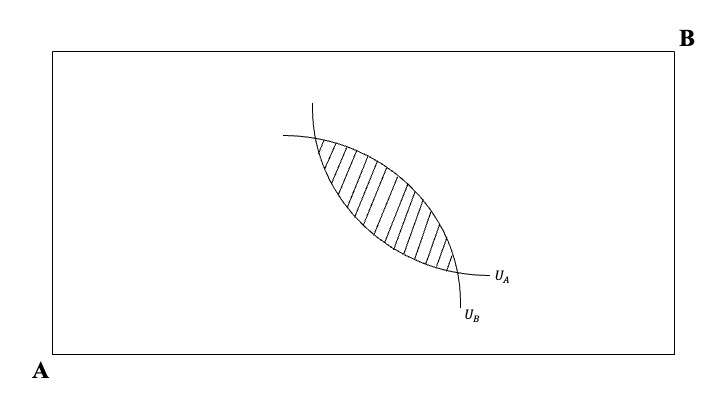
\includegraphics[width=\textwidth]{Figuras/EG Curvas de indiferencias.jpeg}
    \label{fig:caja indiferencias}
\end{figure}

\subsection{Eficiencia y óptimos de pareto}

Dadas las preferencias y dotaciones los individuos podrán intercambiar bienes para maximizar su utilidad. El intercambio se dará si es que hay una posibilidad de mejora para los dos individuos, cuando todas las oportunidades de mejora se hayan agotado nos encontraremos en un óptimo de pareto. Un \textbf{óptimo de Pareto}\marginnote{\textbf{Óptimo de Pareto:} Punto en que las oportunidades de intercambio están agotadas.}[-4cm] graficamente es un punto en la caja de Edgeworth en que no podemos mejorar a un individuo sin empeorar al otro. Este fue un concepto acuñado por \textbf{Vilfredo Pareto}.\marginnote{\textbf{Vilfredo Pareto:} Economista italiano, adopta los equilibrios walrasianos e incorporó a ellos el concepto de óptimo de Pareto.}[-2cm]

Hay que aclarar que estar en un óptimo no es sinónimo de estar en equilibrio, esto tan solo describe una situación en donde no hay intercambios \textit{win-win}. También se puede comentar que estar en un óptimo de pareto no considera las implicaciones morales en cuanto a equidad. Por ejemplo, una dotación inicial esquina donde $A$ ó $B$ concentra todos los recursos cuenta como un óptimo de Pareto.

La manera de saber si un punto es óptimo de Pareto es si la \textbf{tasa marginal de sustitución}\marginnote{\textbf{Tasa marginal de sustitución:} Unidades de un bien que se están dispuestos a renunciar por una unidad marginal del otro bien, manteniendo el mismo nivel de utilidad.}[-1.5cm] para los dos individuos son iguales (condición \ref{eq:TMS=TMS}). La tasa marginal de sustitución se define como las unidades de un bien que pueden cambiar por una unidad de otro bien manteniendo la utilidad constante.
\begin{equation}
    TMS_{x,y}^A = TMS_{x,y}^B \label{eq:TMS=TMS}
\end{equation}
La tasa marginal se calcula como la derivada parcial de la utilidad respecto a un bien divido por la derivada parcial de la utilidad respecto al otro bien. Por lo que podemos expandir la condición \ref{eq:TMS=TMS} como: 
\begin{align*}
    \frac{    \frac{\partial u_A(x,y)}{\partial x}       }{      \frac{\partial u_A(x,y)}{\partial y}     } & =  \frac{    \frac{\partial u_B(x,y)}{\partial x}       }{      \frac{\partial u_B(x,y)}{\partial y}     } 
\end{align*}
La \textbf{curva de contrato} es la colección de puntos óptimos de pareto dentro de la caja de Edgeworth.\marginnote{\textbf{Curva de contrato:} Colección de puntos óptimos de Pareto dentro de la caja de Edgeworth.} A continuación llegamos a la expresión que denotan todos los óptimos de pareto que componen la curva de contrato para los individuos $A$ y $B$. Siendo que el problema para $A$ se plantea como:
\begin{align*}
    \max_{x,y} &\quad u_A(x,y) = x_A^\alpha y_A^{\beta}\quad \\
    \text{s.a.} &\quad p_x \cdot w_{Ax} + p_y \cdot w_{Ay} = p_x \cdot x_A + p_y \cdot y_A
\end{align*}
El problema para $B$ es simétrico\footnote{Cada vez que se diga que un problema es simétrico significa que la solución algebráica seguirá el mismo proceso, por lo que podemos ocupar en este caso el resultado de $A$ para solucionar directamente el resultado de $B$ sin hacer el proceso algebráico de nuevo.}:
\begin{align*}
    \max_{x,y} &\quad u_B(x,y) = x_B^\alpha y_B^{\beta}\quad \\
    \text{s.a.} &\quad p_x \cdot w_{Bx} + p_y \cdot w_{By} = p_x \cdot x_B + p_y \cdot y_B
\end{align*}
Derivamos para obtener la expresión de la tasa marginal de sustitución para ambos individuos. 
\begin{align*}
    TMS_A  = \frac{\alpha x_A^{\alpha -1} y_A^{\beta}}{\beta x_A^\alpha y_A^{\beta -1} } = \frac{\alpha}{\beta} \cdot \frac{y_A}{x_A} \\
    TMS_B= \frac{\alpha x_B^{\alpha -1} y_B^{\beta}}{\beta x_B^\alpha y_B^{\beta -1} } = \frac{\alpha}{\beta} \cdot \frac{y_B}{x_B} 
\end{align*}
Igualamos,
\begin{align*}
    TMS_A = TMS_B \quad \Longrightarrow \quad& \frac{\alpha}{\beta} \cdot \frac{y_A}{x_A} = \frac{\alpha}{\beta} \cdot \frac{y_B}{x_B} \\
   &  \frac{y_A}{x_A} = \frac{y_B}{x_B}
\end{align*}
Es directo entender que,
\begin{align*}
    x_A + x_B = \omega_x \quad 
    y_A + y_B = \omega_y
\end{align*}
Y por tanto aprovechamos para definir nuestra curva de contrato Reemplazando una de aquellas en la expresión anterior.
\begin{align*}
    \frac{y_A}{x_A} &= \frac{\omega_y - y_A}{\omega_x - x_A} \\
    y_A\omega_x &= x_A\omega_y
\end{align*}
Reordenando la expresión,
\begin{equation}
    x_A \cdot \left( \frac{\omega_y}{ \omega_x} \right) = y_A \label{eq:curva de contrato}
\end{equation}
\begin{figure}[htbp]
    \centering
    \caption{Curva de contrato}
    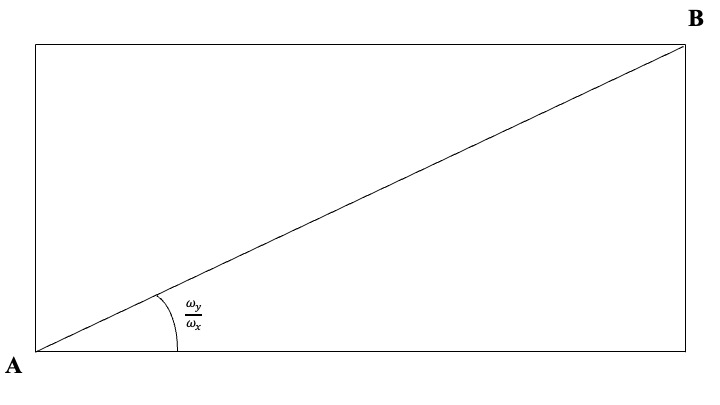
\includegraphics[width=\textwidth]{Figuras/EG Curva de contrato.jpeg}
    \label{fig:diapositiva3}
\end{figure}
Es decir, una dotación que cumpla con la expresión \ref{eq:curva de contrato} pertenece a la curva de contrato y por ende es óptimo de pareto, se agotaron las posibilidades de intercambio por lo que no se puede aumentar la utilidad de uno sin reducir la del otro. La curva de contrato va a tener diferentes formas dependiendo de la función de utilidad de los individuos, en algunos casos no habrá.\footnote{Los gráficos estáran en el anexo.} 

\subsection{Demandas Marshallianas}

Los individuos tendrán una \textbf{demanda marshalliana}\marginnote{\textbf{Demandas Marshallianas:} Son las demandas óptimas resultantes de un problema de maximización sujeto a alguna restricción.} acorde a sus preferencias y riqueza. Para esto el individuo maximiza su utilidad sujeto a una restricción. Si resolvemos el problema para A encontraremos la demanda del individuo para cada bien. En este caso diremos que $\alpha,\beta >0$ y que $\alpha + \beta = 1$
\begin{align*}
    \max_{x,y} &\quad u_A(x,y) = x_A^\alpha y_A^{\beta}\quad \\
    \text{s.a.} &\quad R_A = p_x \cdot x_A + p_y \cdot y_A
\end{align*}
Planteando el lagrangeano,
\begin{equation*}
    \mathcal{L}= x_A^\alpha y_A^{\beta} + \lambda (R_A - p_x \cdot x_A - p_y \cdot y_A)
\end{equation*}
Derivamos las condiciones de primer orden.
\begin{align*}
    \frac{\partial \mathcal{L}}{\partial x_A} = \alpha x_A^{\alpha-1}y_A^\beta - \lambda_x p_x = 0 \quad \quad
    \frac{\partial \mathcal{L}}{\partial y_A} = \beta x_A^\alpha y_A^{\beta -1} - \lambda_y p_y = 0
\end{align*}
Se despejan los lambdas y se igualan las expresiones.
\begin{align*}
    & \lambda_x = \frac{\alpha x_A^{\alpha-1}y_A^\beta }{p_x} \quad 
    \lambda_y = \frac{\beta x_A^\alpha y_A^{\beta-1}}{p_y} \longrightarrow \frac{\alpha x_A^{\alpha-1}y_A^\beta }{p_x} = \frac{\beta x_A^\alpha y_A^{\beta-1}}{p_y} \\
    \text{Reescribiendo,}\quad & x_A = y_A  \left( \frac{p_y \alpha}{p_x \beta} \right)  \quad y_A = x_A \left(  \frac{p_x \beta}{p_y\alpha}  \right)
\end{align*}
El siguiente paso es reemplazar alguna de las expresiones anteriores en la restricción:
\begin{align*}
    p_x\left( y_A\frac{p_y\alpha}{p_x\beta} \right) + p_yy_A = R_A
\end{align*}
Por lo tanto las demandas marshallianas de $A$ serán expresadas como:
\begin{align*}
    y_A^* = \frac{R_A}{p_y} \beta & \quad  x_A^* = \frac{R_A}{p_x} \alpha
\end{align*}
Como el problema es simétrico para $B$ podemos directamente decir:
\begin{align*}
    y_B^* = \frac{R_B}{p_y} \beta & \quad  x_B^* = \frac{R_B}{p_x} \alpha
\end{align*}
Las demandas marshallianas estarán en función de la riqueza, el precio del bien y las preferencias.

\subsection{Precios relativos}

Los precios en esta economía están determinados por la dotación y preferencias y serán tales que todos los mercados estén en equilibrio. Lo que importa no son los los valores absolutos que se les da a los precios sino el el precio de un bien en relación al otro, es por esto que un mismo equilibrio se puede sostener con un vector precios $p=(1,2)$ como con un vector $p=(2,4)$ (si bien los valores absolutos cambiaron, la relación 1 es a 2 sigue presente). Es por esto que al resolver el modelo podemos normalizar uno de los precios a 1, de esta manera  simplificamos el proceso.\footnote{El tener precios numerarios es lo mismo que tomar el vector precios $p = (p_i,p_j)$ y multiplicarlos por $1/p_i$, dejándolos como $p = (1, \frac{p_j}{p_i})$. La gracia está en que tanto la primera expresión del vector como la segunda funcionan para un mismo equilibrio.} 

Para obtener los precios podemos apelar a la ley de Walras y proponer la siguiente expresión,
\begin{equation*}
    x_A^* + x_B^* = \omega_x, \quad \quad y_A^* + y_B^* = \omega_y
\end{equation*}
Tomando el caso del bien $x$ reemplazamos las demandas marshallianas.
\begin{align*}
   \frac{R_A}{p_x} \alpha + \frac{R_B}{p_x} \alpha  &= \omega_x \\
   \frac{\alpha}{p_x} (R_A + R_B) &= \omega_x
\end{align*}
Despejando $p_x$ de esta expresión y (por simetría) expresando también $p_y$.
\begin{align*}
    p_x = (R_A + R_B)\frac{\alpha}{\omega_x}, \quad \quad p_y = (R_A + R_B)\frac{\beta}{\omega_y}
\end{align*}
Lo cual hace sentido, a mayor preferencia por determinado bien mayor es el precio, por otro lado a menor dotación del bien mayor su precio. Por convención diremos que la riqueza total se puede escribir como $R_A + R_B = R = p_x\omega_x + p_y\omega_y$. Dada esta expresión tendremos un problema, todavía no hemos despejado los precios puesto que estos dependen de la riqueza la cual depende recursivamente de los precios. Podemos hacer dos cosas, una de ellas es normalizar uno de los precios a 1, y la otra opción es dividir directamente $p_y/p_x$ para obtener $p_y$ en relación a $p_x$. 

Los precios relativos se pueden expresar entonces como:
\begin{align*}
    \frac{p_y}{p_x} = \frac{ \frac{R\alpha}{\omega_x}  }{  \frac{R\beta}{\omega_y}  } = \frac{\beta \omega_x}{\alpha \omega_y}
\end{align*}
Son las mismas leyes de oferta y demanda, a mayor preferencia de $y$ en relación a $x$ mayor será el precio de $y$ relativo al precio de $x$. 

\subsection{Teoremas del bienestar}

\textbf{Primer teorema del bienestar:} Todo equilibrio walrasiano es óptimo de pareto.

Este teorema plantea que si hay un equilibrio en la economía no habrán oportunidades de intercambio.\footnote{Demostrado en Arrow, Kenneth J. and Gerard Debreu, “Existence of Equilibrium for a Competitive Economy,” Econometrica, 1954.} Este teorema se relaciona fuertemente con la mano invisible en donde cada individuo buscando su propio beneficio llegaría a un punto eficiente. Recordar que para llegar a este equilibrio se tienen que cumplir supuestos bastante fuertes. 

\textbf{Segundo teorema del bienestar:} Todo óptimo de Pareto puede conseguirse mediante un equilibrio walrasiano. 

Para cualquier óptimo de Pareto podemos redistribuir las dotaciones iniciales de manera de conseguir un equilibrio walrasiano. Dada una nueva distribución inicial podemos llegar a un óptimo de Pareto dado mediante el equilibrio walrasiano. 

\subsection{Equilibrio con producción}

Una extensión de lo visto hasta ahora sería considerar que los bienes consumidos se tienen que producir. En este caso las dotaciones no van a ser de bienes sino de factores de producción capital y trabajo ($K,L$). Habrá un total de capital de $\bar{K}$ y un total de trabajo $\bar{L}$, con los que se producen los bienes $x,y$. 

Análogo al consumo la condición de eficiencia para la producción sigue siendo la igualdad entre las tasas marginales, en este caso la \textbf{tasa marginal técnica} (TMT) de sustitución. Es decir, la producción de un bien que podemos intercambiar por la producción adicional de una unidad del otro,
\begin{equation}
    TMT = \frac{ \frac{\partial f(K,L)}{\partial K} }{\frac{\partial f(K,L)}{\partial L} } \label{eq: TMT dfn}
\end{equation}
Dado que se requieren capital y trabajo para los dos bienes estos se tendrán que repartir las dotaciones de manera eficiente, siguiendo \ref{eq: TMT = TMT}.
\begin{equation}
    TMT^x_{K,L} = TMT^y_{K,L} \label{eq: TMT = TMT}
\end{equation}
Podemos formar una caja de Edgeworth de producción como se puede ver en la figura \ref{fig:diapositiva4}.
\begin{figure}[htbp]
    \centering
    \caption{Caja de Edgeworth en la producción}
    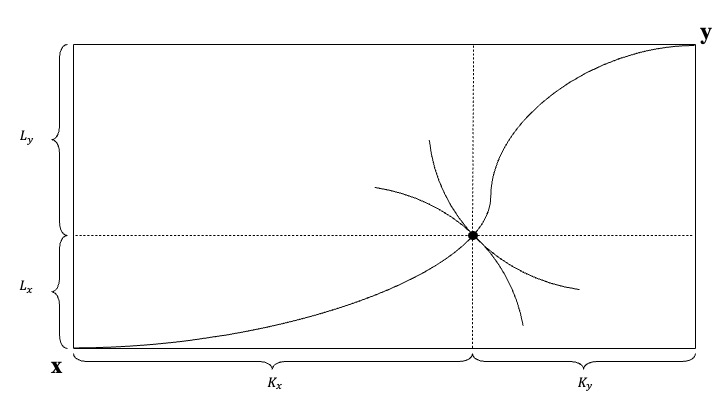
\includegraphics[width=\textwidth]{Figuras/EG Curva de contrato con produccion.jpeg}
    \label{fig:diapositiva4}
\end{figure}
Las curvas de contrato se relacionan con las fronteras de posibilidades. La \textbf{frontera de posibilidades}\marginnote{\textbf{Frontera de posibilidades:}} es una curva que describe todos los puntos en donde se ocupan eficientemente los factores productivos para producir dos bienes, es decir, son los puntos factibles donde no es posible aumentar la producción de un bien sin disminuir la producción del otro. En la figura \ref{fig:diapositiva5} se observan dos puntos, uno que está ubicado en la curva es eficiente y otro que no es eficiente puesto que se puede producir más de un bien sin disminuir la producción de otro. Como todos los puntos de la curva de contrato satisfacen la condición de eficiencia se puede decir que también pertenecen a la curva de contrato.
\begin{figure}[htbp]
    \centering
    \caption{Frontera de posibilidades de producción}
    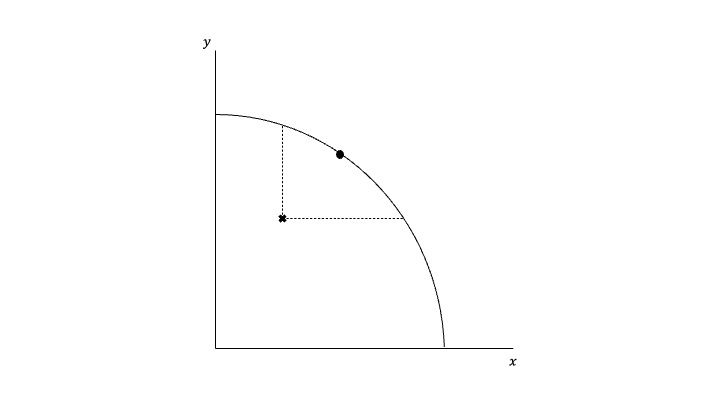
\includegraphics[width=\textwidth]{Figuras/EQ Frontera de posibilidades de produccion.jpeg}
    \label{fig:diapositiva5}
\end{figure}
Para más detalle puede leer el anexo.